% \documentclass[10pt, conference, compsocconf]{IEEEtran}
%\documentclass[conference]{IEEEtran}
\documentclass[letter]{sig-alternate}
\usepackage{eso-pic,xcolor}
\makeatletter
%
\pdfpagewidth=8.5in
\pdfpageheight=11in
\usepackage{flushend}
%\AddToShipoutPicture*{%
%\setlength{\@tempdimb}{20pt}%
%\setlength{\@tempdimc}{\paperheight}%
%\setlength{\unitlength}{1pt}%
%\put(\strip@pt\@tempdimb,\strip@pt\@tempdimc){%
%   \makebox(0,-60)[l]{\color{blue}%
%
%  }%
  
%\put(\strip@pt\@tempdimb,\strip@pt\@tempdimc){%
%    \makebox(0,-85)[l]{\color{black}%
%}%
%}%

%\put(\strip@pt\@tempdimb,\strip@pt\@tempdimc){%
%    \makebox(0,-110)[l]{\color{black}%
%}%
%  }%
%}

%
\def\ps@headings{%
\def\@oddhead{\mbox{}\scriptsize\rightmark \hfil \thepage}%
\def\@evenhead{\scriptsize\thepage \hfil \leftmark\mbox{}}%
\def\@oddfoot{}%
\def\@evenfoot{}}
\makeatother




\pagestyle{headings}

\title{Next-NDNVideo: live and pre-recorded streaming \\\ using Consumer / Producer API over NDN}

\author{
%Paper \#231, 13 pages
Lijing Wang \\ {\normalsize Tsinghua University} \\ {\normalsize wanglj11@mails.tsinghua.edu.cn }
\and Ilya Moiseenko \\ {\normalsize UCLA} \\ {\normalsize iliamo@cs.ucla.edu }
\and Lixia Zhang \\ {\normalsize UCLA} \\ {\normalsize lixia@cs.ucla.edu }
}


\newfont{\nicettfont}{cmtt10}
\newcommand{\ndnName}[1]{``{\nicettfont #1}''}
\renewcommand{\texttt}[1]{{\nicettfont #1}}

\newcommand{\todo}[1]{\vspace{2 mm}\par \noindent \marginpar{\textsc{ToDo}}
\framebox{\begin{minipage}[c]{0.95 \columnwidth}
\tt #1 \end{minipage}}\vspace{5 mm}\par}

\usepackage{graphicx}
% \usepackage[colorlinks]{hyperref}
\usepackage[]{hyperref}
\usepackage{breakurl}
\usepackage{url}
\usepackage[nocompress]{cite}
\usepackage{amsmath}
% \usepackage{verbatim}
% \usepackage{algpseudocode}
\usepackage{algpseudocode,algorithm}
% More customizeable version. Probably it would be better to convert pseudocode to 2e format
% \usepackage{algorithm2e} 
\usepackage{multirow}
\usepackage{times}
\usepackage{color}

\graphicspath{{figures/}}

\begin{document}

\maketitle

% \begin{abstract}
% Named Data Networking (NDN) is a general purpose protocol offering rich functionality at the network layer: caching, multi-path forwarding, multicast delivery, and data-based security model. Above the network layer, system libraries simplify application developers' tasks by providing an easy to use yet powerful API to utilize the functions enabled by NDN.  This paper presents the design of a Consumer / Producer programming interface that supports application level framing via new data retrieval protocols, and several supporting mechanisms to make NDN application programming easier and faster.
% \end{abstract}


%\begin{IEEEkeywords}
%Information-centric networks, named data networking, API, inter-process communication
%\end{IEEEkeywords}
\input{01introduction}
%!TEX root = nextndnvideo-tr.tex
\section{background} % (fold)
\label{sec:background}
\subsection{Consumer / Producer API}
Consumer-Producer API~\cite{api-tr} provides a generic programming interface to NDN communication protocols and architectural modules. A consumer context associates an NDN name prefix with various data fetching, transmission, and content verification parameters, and integrates processing of Interest and Data packets on the consumer side. A producer context associates an NDN name prefix with various packet framing, caching, content-based security, and namespace registration parameters, and integrates processing of Interest and Data packets on the producer side.

In NDNlive and NDNtube, the video publisher consists of multiple producers generating video and audio frames separately. The corresponding video players consist of multiple consumers sending Interests for the video and audio frames. Consumer / Producer API simplifies the application logic at both sides: media production and media consumption. Since video frames are too large to be encapsulated by a single Data packet, the media production pipeline has to include a content segmentation step in order to split the content into multiple Data packets. Producer API provides this segmentation functionality. At the same time, since a video frame cannot be retrieved by a single Interest packet, UDR and RDR protocols behind the Consumer API automatically pipeline Interest packets and solve other tasks related to the retrieval of the application frame. 
%In the case of MPEG-DASH, all these low-level details are handled by the HTTP / TCP protocol machinery. 
We will talk about the implementation details in Section~\ref{sec:implementation}.

\subsection{Gstreamer}

We use Gstreamer~\cite{gstreamer} to handle the media processing part. 

In NDNLive, raw video images captured by the camera are transferred to the \textit{Encoder\_v} component and are encoded into \textit{H264} format. Then the encoded video is passed to the \textit{Parser\_v} to be parsed into frames (\textit{B, P or I frame}). The microphone captures the raw audio, which is passed to the \textit{Encoder\_a}. The encoder component encodes the raw audio into \textit{AAC} format. The encoded audio stream is transferred to the \textit{Parser\_a} to be parsed into audio frames, which are passed to the Producer API for any possible segmentation. Video and audio data is retrieved frame by frame that are passed to the video \textit{Decoder\_v} and audio \textit{Decoder\_a} for the decoding into the format which the video \textit{Player\_v} or audio \textit{Player\_a} can play.

In NDNTube, the source for video and audio streams is an mp4 file containing \textit{H264} video and \textit{AAC} audio. Gstreamer opens the file and passes it to the \textit{Demuxer} component to separate video and audio streams. Since the video file is already encoded, the media processing pipeline does not have an \textit{Encoder} component in it. The encoded video or audio streams are separately pushed into the \textit{Parser} to generate video and audio frames.

%Because we need to extract the frames from the video source, so now we only support \textit{H264} video encoded format and  encoded format for NDNLive and \textit{MP4} file format for NDNTube. 

\subsection{Repo-ng}
NDNLive streams the captured video and audio non-stop. Therefore, the media publisher just keeps producing new frames and does not care about the data it produced several minutes ago. The consumer is also interested only in recent video and audio frames. As long as the producer is attached to the NDN network, it  will serve the incoming Interests. %The consumer can get the data back and play them back immediately.

NDNTube publishes the video only once --- all Data packets corresponding to audio and video frames are permanent and never change after the initial publication. Since the same video could be requested multiple times by different users, it is reasonable to store the produced Data packets in a `database' which is exposed to the requests from the network. Otherwise, every time a different user requests the same video, the corresponding video and audio Data packets would have to be republished (and signed) in case NDN cache has not been able to satisfy these Interests.

Repo-ng~\cite{repo-ng} is used as a permanent storage for the video and audio content. Repo-ng (repo-new generation) is an implementation of NDN persistent in-network storage, which exposes a Repo protocol~\cite{Repo-Protocol} allowing write access to applications. Repo insertion is natively supported by the Producer API with \textit{LOCAL\_REPO} option (if repo is running on the local host) or \textit{REMOTE\_REPO\_PREFIX} option to point to the right remote repo by its name prefix. 
% section section_name (end)
%!TEX root = nextndnvideo-tr.tex
\vspace{0.3cm}
\section{design} % (fold)
\label{sec:design}
\subsection{Architecture}
Next-NDNVideo is based on Consumer / Producer API over Named Data Networking. It contains two kinds of roles - producer and consumer. The whole architecture (Figure~\ref{fig:arch}) is described below.

\begin{figure*}%[htbp]
  \centering
  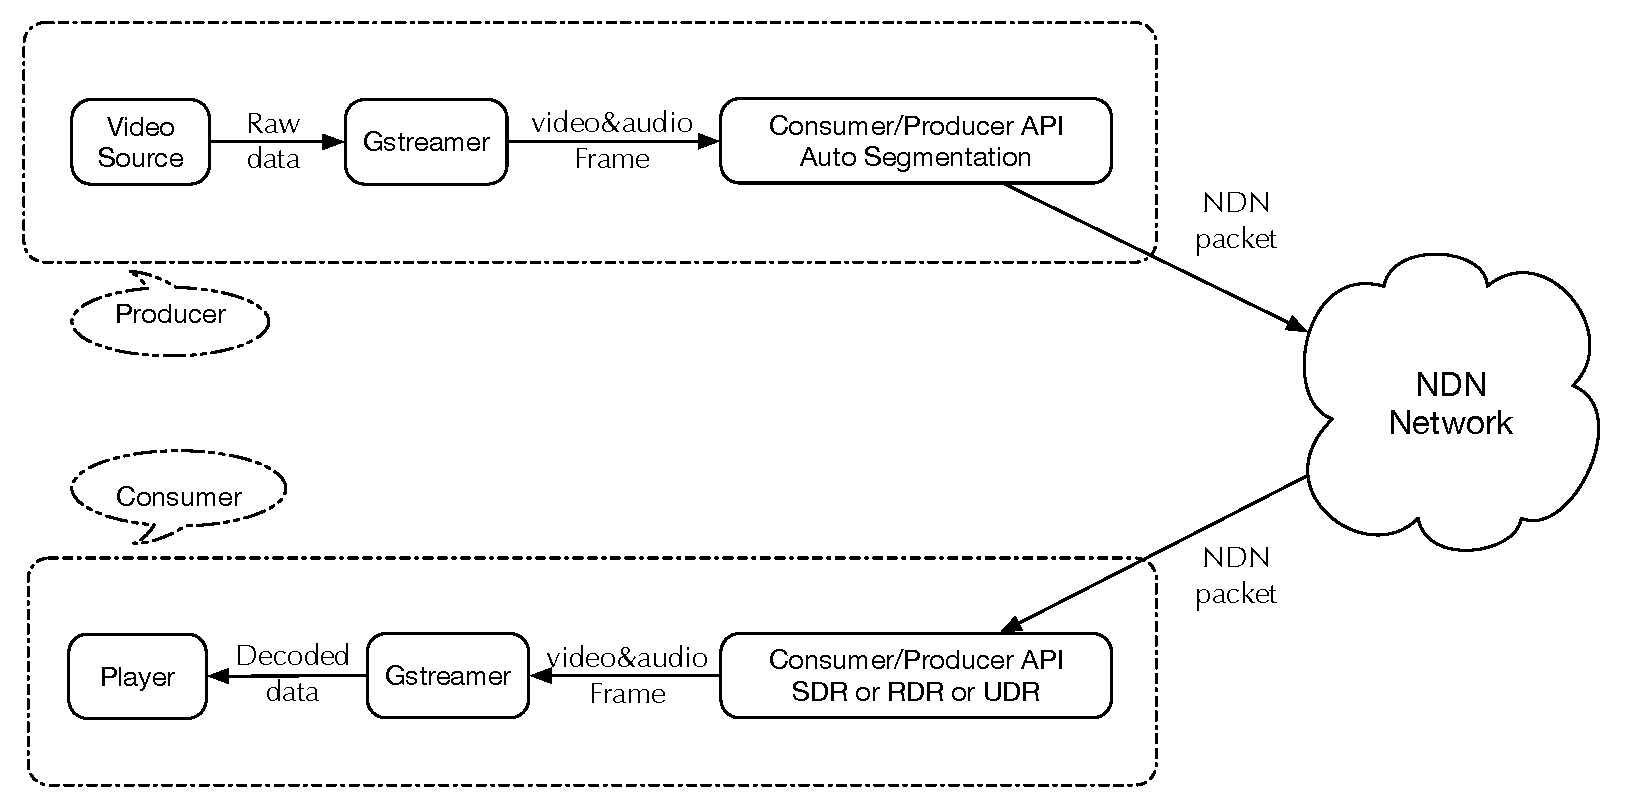
\includegraphics[scale=0.55]{architecture}
  % \vspace{-0.3cm}
  \caption{Architecture of Next-NDNVideo}
  \label{fig:arch}
  %\vspace{-0.2cm}
\end{figure*}

The producer is responsible for generating video and audio streaming. It behaves as the content publisher. We use Gstreamer to extract the video and audio frames from video source. Then we call Consumer / Producer API to encapsulate the data frames into NDN packets. In this case these NDN packets are available to fetch. The producer part can work even without being attached to the NDN network. The producer's packages will be cached in the \textit{Send Buffer} the API maintained and \textit{Content Store} of NFD\cite{nfd-guide}. Also the NDN packets can be written into Repo\cite{repo-ng}. Then Repo will take charge of satisfying the data request.

Every time the consumer wants to play back some video, it should send interests to fetch the data by using one of the Data Retrieval Protocol \textit{(SDR/UDR/RDR)}. When Consumer / Producer API brings data back, the call back function will be triggered to retrieve data. The reassembled video or audio frame will be passed to Gstreamer for further processing. Finally, Gstreamer will provide the decoded data to video player for playing back. Because all NDN applications are interest-driven, only the consumer keeps sending interest, it can fetch the data and play it back.

According to the content generating and data retrieval pattern, Next-NDNVideo can be divided into two different implementations. One is Live Streaming, which the producer captures video from camera and audio from microphone and keeps publishing them as a live stream. Any time the consumer sends interest asking for the video stream, it will get the latest video and audio. Another is Pre-recorded Streaming, which is more like youtube. In this case the consumer can send interest asking for the latest playing list and chose one to play. The video and audio frames associated with one video file will be written into Repo in advance. The producer only needs to keep publishing the latest playing list containing all the names of video files that are ready to play.

\subsection{Naming Structure}
Next-NDNVideo produces video and audio stream separately. Every single frame will form a piece of data, so they need a unique name. And before consuming the video and audio content, it should first use the stream information to set up the playing pipeline. The following is an example name of Pre-recorded Streaming. 
\begin{quote}
``/ndn/ucla/recordvideo/video-1234/video/content \\\ /8/\%00\%00''
\end{quote}
\begin{itemize}
	\item{\textbf{Routing Prefix:}} ``/ndn/ucla/recordvideo'' is the prefix.
	\item{\textbf{Video Name:}} ``/video-1234'' is a representation for one specific video such as file name.
	\item{\textbf{Video Mark:}} ``/video'' is a mark to distinguish video and audio.
	\item{\textbf{Streaminfo Mark:}} ``/content'' represents the frames and ``/streaminfo'' represents the stream information.
	\item{\textbf{Frame Number:}} ``/8'' is frame number, which Streaminfo does not have this component.
	\item{\textbf{Segment Number:}} ``\%00\%00'' is the segment number. Because most video frames would contain more than one segment, this component is essential. As we mentioned before the Consumer / Producer API will do the segmentation processing, so the segment number will be appended by the API automatically. Streaminfo does not have this component, neither.
\end{itemize}

Then we can conclude that the above name stands for a piece of data which is the segment 0 inside the 8th video frame of video-1234 under the prefix of /come/youtube. The relative stream information name is as following.
\begin{quote}
``ndn/ucla/recordvideo/video-1234/video/streaminfo \\\ /pipeline''
\end{quote}

Except for the last component, the others are all introduced above. The last component of Streaminfo is the information type.
\begin{itemize}
	\item{\textbf{Info Type:}} 
	\begin{itemize}
		\item{\textbf{pipeline:}} means that it asks for essential information to set up the playing back pipeline. 
		\item{\textbf{current\_id:}} means that it asks for the current frame number of this video. This is used only by NDNLive.
		\item{\textbf{final\_id:}} means that it asks for the final frame number of this video. This is used only by NDNTube. 
	\end{itemize}
\end{itemize}


% \begin{figure}%[htbp]
%   \centering
%   \includegraphics[scale=0.5]{listnaming}
%   % \vspace{-0.3cm}
%   \caption{NDN packet types.}
%   \label{fig:listnaming}
% \end{figure}

% section section_name (end)
%!TEX root = nextndnvideo-tr.tex
\section{implementation} % (fold)
\label{sec:implementation}
Next-NDNVideo is developed using Consumer / Producer API over NDN. This API is an modification version of ndn-cxx library and requires NFD running to forward interests. To compact with Consumer / Producer API and NFD, the project is also written in C++. We use Gstreamer 1.4.3 (other branch not tested) to process media. The supporting platform is UNIX-Like such as Mac OS and Linux. We will explain the implementation details about Live Streaming and Prerecorded respectively.
\begin{figure}[htbp]
  \centering
  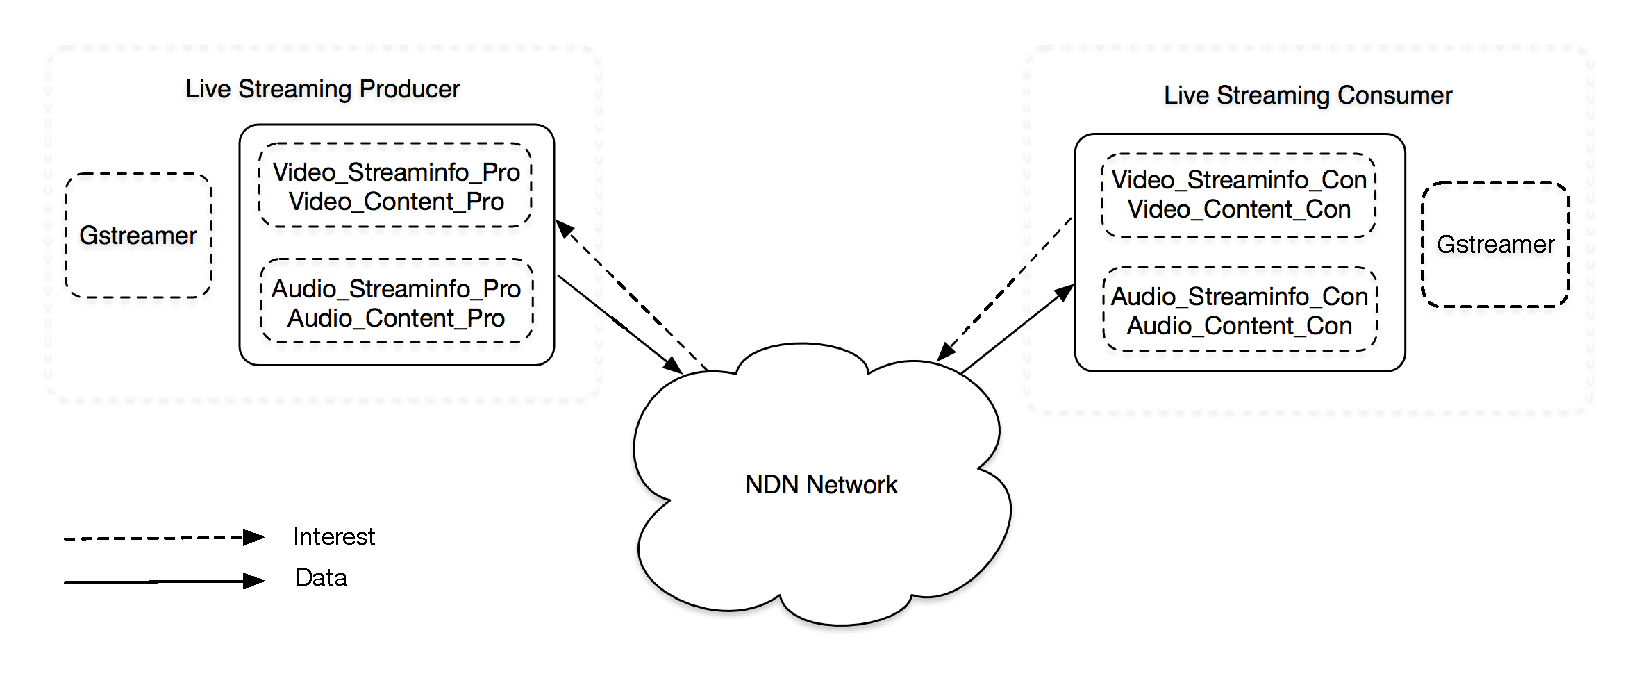
\includegraphics[scale=0.3]{live_arch}
  % \vspace{-0.3cm}
  \caption{Live Streaming Architecture}
  \label{fig:live_arch}
  %\vspace{-0.2cm}
\end{figure}

\subsection{Live Streaming}
The architecture of Live Streaming is shown as Figure~\ref{fig:live_arch}. It has four producers: video stream information producer, video content producer, audio stream information producer and audio content producer. Before the consumer asks for the true video data, it must fetch the live stream information to set up the Gstreamer playing pipeline. The stream information includes frame rate, width, height, stream format and so on. For Live streaming, to inform consumer of the starting frame number the producer also need to produce the latest frame number if requested. The video and audio are produced and consumed separately, so they must be in separate thread. In both (producer and consumer) side, the Gstreamer should keep running in the background, so Gstreamer needs another thread. To conclude, in each side we have three threads running at the same time. Components inside one black dotted rectangle belong to the same thread.

The following part will describe some details about media processing, the data retrieval protocols we use and the pseudo code.
\subsubsection {Media Precessing}
\paragraph {Producer}
The producer will capture video from camera and audio from microphone, then produce them frame by frame. The progressing detail is shown as Figure~\ref{fig:live_detail}.

\begin{figure*}%[htbp]
  \centering
  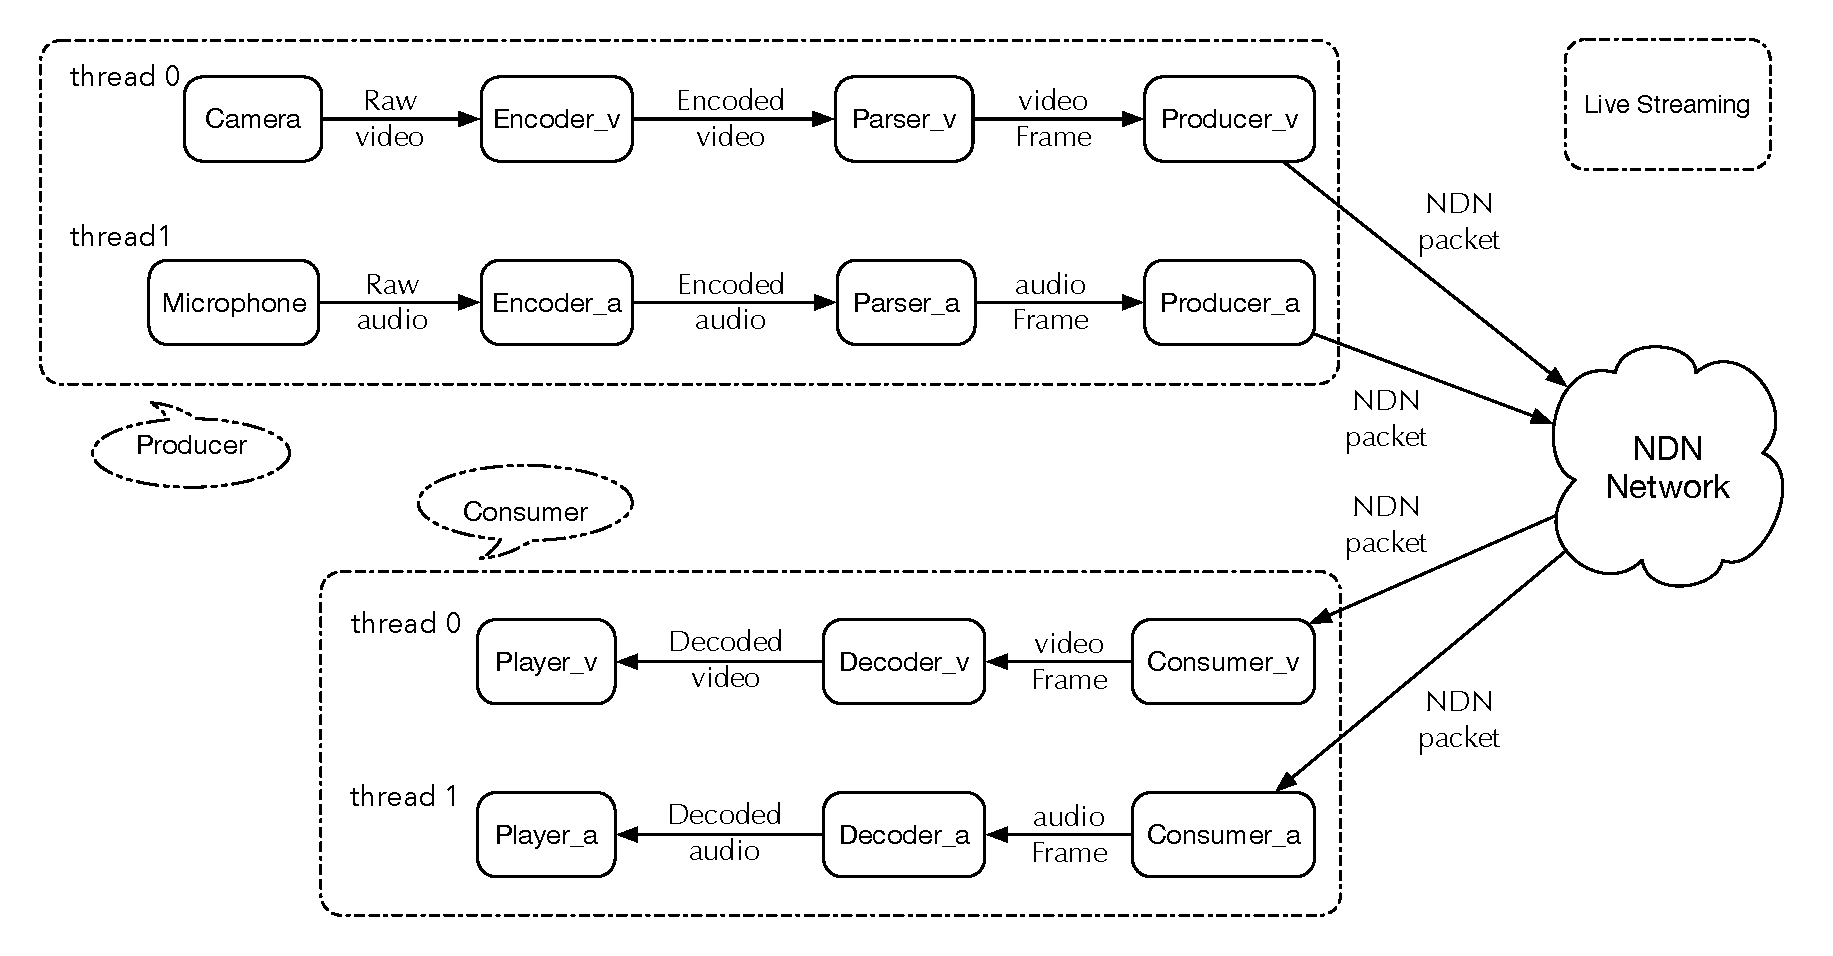
\includegraphics[scale=0.55]{live_detail}
  % \vspace{-0.3cm}
  \caption{Live Streaming Media Processing}
  \label{fig:live_detail}
  %\vspace{-0.2cm}
\end{figure*}

The raw video pictures captured by camera would be transferred to \textit{Encoder\_v} component and will be encoded into \textit{H264} format. Then the encoded video is transmitted into \textit{Parser\_v} to be parsed into frames (\textit{B, P or I frame}). The last component is the \textit{Producer\_v}, which is in charge of producing video frame by frame.

For audio, the microphone will capture the audio then push the raw audio into \textit{Encoder\_a}. The encoder component will encode the raw audio into \textit{ACC} format. The encoded audio stream will be transferred to \textit{Parser\_a} to get parsed then passed to \textit{Producer\_a} component. Finally, this audio producer will produce the audio frame by frame.

\paragraph {Consumer}
The consumer also processes video and audio separately.

For video, the \textit{Consumer\_v} component keeps sending interests to fetch the video data. And it will get data retrieved frame by frame. Then the video frame will be thrown to the \textit{Decoder\_v} to get decoded into the format which the \textit{Player\_v} can play it back.
For audio, the \textit{Consumer\_a} component fetches the audio data by sending audio interests. The retrieved audio frame will be transferred to \textit{Decoder\_a} to get decoded. The decoded audio will be sent to \textit{Player\_a}. At the end, the \textit{Player\_v} and \textit{Player\_a} should play video and audio together.

\paragraph {Synchronization between video and audio}
\label{par:sync}
Since we process video and audio separately, it is a vital problem to keep them synced. Gstreamer can handle the synchronization for us in this way:

When video and audio are captured, they are timestamped by the Gstreamer. The time information will be recorded in \textit{GstBuffer} data structure which Gstreamer used to contain media data. This time information will also be transferred along with video or audio frame. Then when the consumer fetches the video or audio frame separately. The video and audio frames will be pushed into the same \textit{GstQueue}. Gstreamer will extract the timestamps hiding in the video and audio frames, then play them back together according to the timestamps.

\subsubsection{Data Retrieval Protocol}
\paragraph{Streaminfo Retrieval} % (fold)
\label{par:streaminfo}
Because the stream information contains only one segment and will be fetched only one time (at the beginning of the playing back). We use \textbf{SDR} (\textit{Simple Data Retrieval}) to fetch the stream info for video and audio. Except for the basic stream information, the consumer also needs to obtain the current frame number the producer just produced. So that the frame consumer can start from this frame number and increase it one by one. To retrieve the latest stream information, \textit{Right\_Most\_Child} option should be set as TRUE.
\paragraph{Frames Retrieval} 
Considering about the situation of live streaming, the consumer part needs to keep the video and audio retrieving progress running all the time. The aim is to fetch all the segments inside one frame as soon as possible. The fetching process should NOT be blocked because of one segment missing. So we use \textbf{UDR} (\textit{Unreliable Data Retrieval}) for frames retrieval of living streaming. Then the consumer part should take care of the segments reassemble and ordering stuff.

\subsubsection{Pseudocode}

\begin{algorithm}%[hbtp]
\caption{Live video producer}
\label{alg:liveproducer}
\begin{algorithmic}[1]
\State $h_v \leftarrow $ \textbf{producer}(/ndn/ucla/livevideo/video/)
\State \textbf{setcontextopt}($h_v$, \textbf{cache\_miss}, \textit{ProcessInterest})
\State \textbf{attach}($h_v$)
\vspace{0.2cm}
	\While{\textit{TRUE}}
	\State $Name \textbf{ } suffix_v \leftarrow $ video frame number
	\State $content_v \leftarrow $ video frame captured from Camera
	\State \textbf{produce}($h_v$, $Name\textbf{ }suffix_v$, $content_v$)
	\EndWhile
\vspace{0.2cm}
\vspace{0.2cm}
\State $h_a \leftarrow $ \textbf{producer}(/ndn/ucla/livevideo/audio/)
\State \textbf{setcontextopt}($h_a$, \textbf{cache\_miss}, \textit{ProcessInterest})
\State \textbf{attach}($h_a$)
\vspace{0.2cm}
	\While{\textit{TRUE}}
	\State $Name \textbf{ } suffix_a \leftarrow $ audio frame number
	\State $content_a \leftarrow $ audio frame captured from mirophone
	\State \textbf{produce}($h_a$, $Name\textbf{ }suffix_a$, $content_a$)
	\EndWhile
\vspace{0.4cm}
\Function{ProcessInterest}{Producer \textbf{h}, Interest \textbf{i}}
  \If{\textit{NOT Ready}}
    \State $appNack \leftarrow $ \textbf{AppNack}($i$, \textbf{RETRY-AFTER})
    \State \textbf{setdelay}($appNack$, $estimated\_time$)
    \State \textbf{nack}($h$, $appNack$)
  \EndIf
   \If{\textit{Out of Date}}
    \State $appNack \leftarrow $ \textbf{AppNack}($i$, \textbf{NO-DATA})
    \State \textbf{nack}($h$, $appNack$)
  \EndIf
\EndFunction
\end{algorithmic}
\end{algorithm}

There are two situations we should consider carefully. The first one is that, because once the consumer started consuming frames, it will have no idea the about the current frame number which producer is producing. It may sometimes request for a frame number ahead of the producing. It is the producer's duty to inform the consumer about such knowledge. We introduce \textbf{NACK}(\textit{Negative Acknowledgment}) to handle such situation. 

For example, in Algorithm~\ref{alg:liveproducer} , when the interest asks for a piece of data not existing (out of date or not be produced yet), this will trigger the \textit{cache\_miss} callback function (\textit{Process\_Interest}). In that function, if the data was not produced (\textit{not\_ready}), the producer will set up an \textit{APPLICATION\_NACK} with \textit{PRODUCER\_DELAY} option for this interest together with the estimated delay time.

At the same time, although before the consumer starts to consume frames, it will ask for the current number. Such information may also go out of date because of the network delay. These out-of-date frames will never be produced again, because the streaming is live. When faced with such situation, the producer will simply send a \textbf{NACK} with \textit{NO-DATA} option.

\begin{algorithm}[hbtp]
\caption{Live video consumer}
\label{alg:liveconsumer}
\begin{algorithmic}[2]
\State $h_v \leftarrow $ \textbf{consumer}(/ndn/ucla/livevideo/video/, \textit{UDR})
%\State \textbf{setcontextopt}($h_v$, \textit{EMBEDDED\_MANIFESTS}, \textit{TRUE})
%\State \textbf{setcontextopt}($h_v$, \textbf{receive\_buffer\_size}, 1MB)
\State \textbf{setcontextopt}($h_v$, \textbf{new\_segment}, \textit{ReassambleVideo})
\vspace{0.2cm}
	\While{\textit{TRUE}}
	\State $Name \textbf{ } suffix_v \leftarrow $ video frame number
	\State \textbf{consume}($h_v$, $Name\textbf{ }suffix_v$)
	\State $framenumber ++$
	\EndWhile
\vspace{0.2cm}

\Function{ReassambleVideo}{Data \textbf{segment}}
    \State $content \leftarrow $ reassamble \textbf{segment}
    \If{\textit{Final\_Segment}}
		\State $video \leftarrow $ decode \textbf{content}
	   	\State Play $video$
	\EndIf
\EndFunction

\vspace{0.4cm}

\State $h_a \leftarrow $ \textbf{consumer}(/ndn/ucla/livevideo/audio/, \textit{UDR})
\State \textbf{setcontextopt}($h_a$, \textbf{new\_segment}, \textit{ReassambleAudio})
\vspace{0.2cm}
	\While{\textit{NOT EOS}}
	\State $Name \textbf{ } suffix_a \leftarrow $ audio frame number
	\State \textbf{consume}($h_a$, $Name\textbf{ }suffix_a$)
	\State $framenumber ++$
	\EndWhile
\vspace{0.2cm}

\Function{ReassambleAudio}{Data \textbf{segment}}
%   \State $video \leftarrow $ decode \textbf{content}
    \State $content \leftarrow $ reassamble \textbf{segment}
    \If{\textit{Final\_Segment}}
		\State $audio \leftarrow $ decode \textbf{content}
	   	\State Play $audio$
	\EndIf
\EndFunction
\end{algorithmic}
\end{algorithm}

\subsection{Pre-recorded Streaming}
\begin{figure}%[htbp]
  \centering
  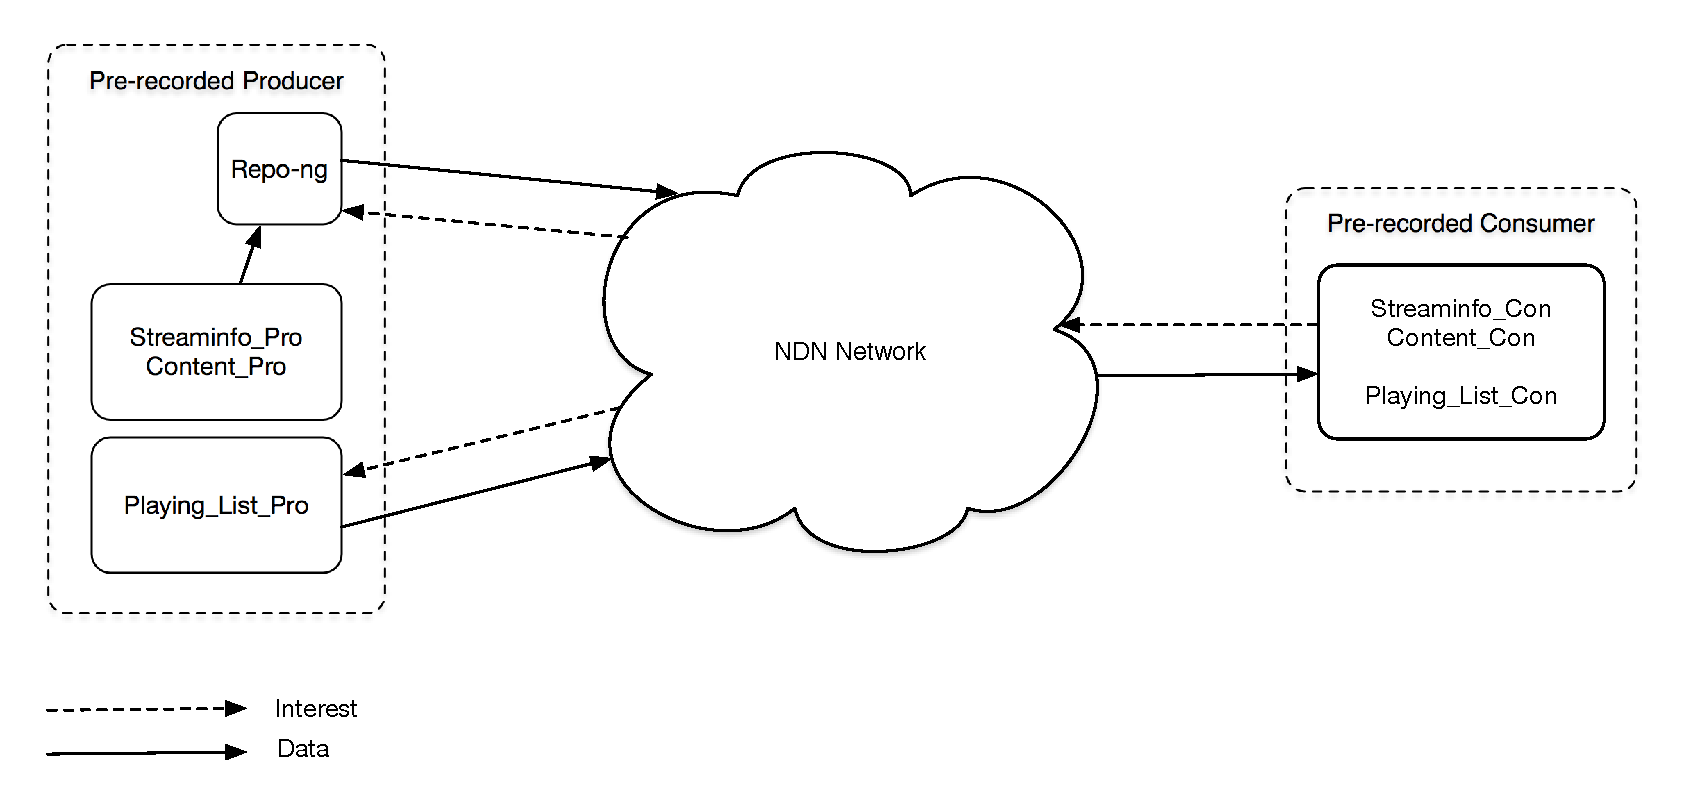
\includegraphics[scale=0.3]{record_arch}
  % \vspace{-0.3cm}
  \caption{Playing List Naming}
  \label{fig:record_arch}
  %\vspace{-0.2cm}
\end{figure}

The Pre-recorded Streaming architecture is slightly different from Live Streaming (Figure~\ref{fig:record_arch}). Firstly, \textbf{Repo-ng} is added in the producer side to provide the constant storage for video and audio data. Secondly, the playing list producer and consumer are introduced. This producer is to produce the playing list, which records the video names in one specific directory of producer. Because the video files could be added or deleted anytime, every time the producer detected the change of the directory, it will produce a new playing list with the same name except for appending a new timestamp. Figure~\ref{fig:list_naming} is one list naming example. 

\begin{figure}%[htbp]
  \centering
  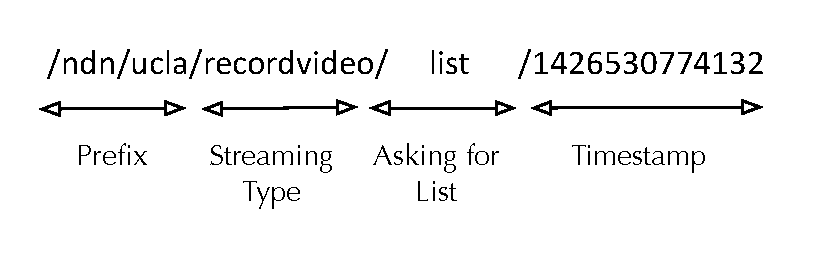
\includegraphics[scale=0.5]{list_naming}
  % \vspace{-0.3cm}
  \caption{Pre-recorded Streaming Architecture}
  \label{fig:list_naming}
  %\vspace{-0.2cm}
\end{figure}

The other two producers are almost the same with Live Streaming. One producer produces the stream information of the recorded video. The other takes charge of producing the frames. The difference is that the stream info and frame data will be inserted into \textbf{Repo-ng}, but not attached to the NDN Network. Because different from live streaming, the pre-recorded video is permanent. Once the data was produced and the same data could be requested many times. However, for the live streaming, it just keeps producing and doesn't care about the data it produced several minutes ago. So the video file should be only produced once then written into Repo-ng and should not be produced again. The Repo-ng will respond to the interests. This can also relieve the producing pressure of producer.  

The consumer part should send interests to request the playing list in advance. Only after the consumer has the knowledge of all the files which producer has, it can ask for one specific video to play back. Same as live streaming, the pre-recorded video consumer also needs to retrieve the \textit{Streaminfo} of the video file to set up the playing pipeline of Gstreamer. Then the consumer keeps sending video and audio content retrieval interest with the frame number increased one by one. One difference from live streaming is that, the pre-recorded consumer must know the ending frame of the video file. So except for the basic information of pipeline, it should contain the final video and audio frame id. Then the consumer can know when to stop sending interests. On the contrary, the live streaming consumer just keep increasing the frame number until user close it. Because the video is alive and will be producing all the time. But the live streaming needs to obtain the current frame number to follow the step with the producer. The pre-recorded video consumer does not have this part.

\paragraph{Media Processing}

The main difference from live streaming is the video source. The pre-recorded video source is the video file. Gstreamer should first read video file then pass it to the \textit{Demuxer} component to separate video and audio stream. Because the video file is already encoded, so there is no \textit{Encoder} component here. The separate encoded video or audio is pushed into the \textit{Parser} to generate frames. The frames will be produced by Consumer / Producer API and inserted into \textit{Repo-ng}. The API will handle the segmentation automatically. The media processing of consumer part is the same with live streaming.

There also exists the synchronization problem between video and audio. As we describe above~\ref{par:sync}, the Gstreamer will handle the synchronization part as long as we give the video and audio frame correct timestamps. In live streaming, it is the capturing component who stamps the frames. In pre-recorded streaming, it is the \textit{Dumxer} who is responsible for time stamping. Once the media data flows through \textit{Dumxer}, this component will separate the video stream and audio stream according to their file type such as \textit{MP4} and adding the time information in each \textit{GstBuffer}.

\paragraph{Data Retrieval}
Same with \textit{Streaminfo} tetrieval of live streaming, we use \textbf{SDR} to retrieve stream information and the playing list. We want to fetch the latest version of playing list, so we should set \textit{Right\_Most\_Child} option as TRUE as well.

However, for the frames retrieval, we should use \textbf{RDR} (\textit{Reliable Data Retrieval}). Because we can't stand any segment missing for the recorded video, we always want the good quality of video and audio. If the video segments are not received on time the \textit{Buffering} mechanism will be triggered. Only when Gstreamer accumulates enough video and audio frames (such as two seconds duration) it will continue to play back. Otherwise, it will be just paused until the buffer is full.

\paragraph{Pseudocode}

\begin{algorithm}[hbtp]
\caption{Pre-recorded video publisher}
\label{alg:recordproducer}
\begin{algorithmic}[3]
\State $h_v \leftarrow $ \textbf{producer}(/ndn/ucla/recordvideo/video-1234/

video/)
\State \textbf{setcontextopt}($h_v$, \textbf{repo\_prefix}, \textit{/ndn/ucla/repo})
\vspace{0.2cm}
	\While{\textit{NOT EOF}}
	\State $Name \textbf{ } suffix_v \leftarrow $ video frame number
	\State $content_v \leftarrow $ video frame
	\State \textbf{produce}($h_v$, $Name\textbf{ }suffix_v$, $content_v$)
	%\State $framenumber ++$
	\EndWhile
\vspace{0.2cm}
\vspace{0.2cm}
\State $h_a \leftarrow $ \textbf{producer}(/ndn/ucla/recordvideo/video-1234/

audio/)
\State \textbf{setcontextopt}($h_a$, \textbf{repo\_prefix}, \textit{/ndn/ucla/repo})
\vspace{0.2cm}
	\While{\textit{NOT EOF}}
	\State $Name \textbf{ } suffix_a \leftarrow $ audio frame number
	\State $content_a \leftarrow $ audio frame
	\State \textbf{produce}($h_a$, $Name\textbf{ }suffix_a$, $content_a$)
	%\State $framenumber ++$
	\EndWhile
\end{algorithmic}
\end{algorithm}

\begin{algorithm}[hbtp]
\caption{Pre-recorded video consumer}
\label{alg:recordconsumer}
\begin{algorithmic}[4]
\State $h_v \leftarrow $ \textbf{consumer}(/ndn/ucla/recordvideo/video-1234/

video/, \textit{RDR})
%\State \textbf{setcontextopt}($h_v$, \textit{EMBEDDED\_MANIFESTS}, \textit{TRUE})
%\State \textbf{setcontextopt}($h_v$, \textbf{receive\_buffer\_size}, 1MB)
\State \textbf{setcontextopt}($h_v$, \textbf{new\_content}, \textit{ProcessVideo})
\vspace{0.2cm}
	\While{\textit{NOT EOS}}
	\State $Name \textbf{ } suffix_v \leftarrow $ video frame number
	\State \textbf{consume}($h_v$, $Name\textbf{ }suffix_v$)
	\State $framenumber ++$
	\EndWhile
\vspace{0.2cm}

\Function{ProcessVideo}{byte[] \textbf{content}}
   \State $video \leftarrow $ decode \textbf{content}
%   \State $audio \leftarrow $ decode \textbf{content}
   \State Play $video$
\EndFunction

\vspace{0.4cm}

\State $h_a \leftarrow $ \textbf{consumer}(/ndn/ucla/recordvideo/video-1234/

audio/, \textit{RDR})
\State \textbf{setcontextopt}($h_a$, \textbf{new\_content}, \textit{ProcessAudio})
\vspace{0.2cm}
	\While{\textit{NOT EOS}}
	\State $Name \textbf{ } suffix_a \leftarrow $ audio frame number
	\State \textbf{consume}($h_a$, $Name\textbf{ }suffix_a$)
	\State $framenumber ++$
	\EndWhile
\vspace{0.2cm}

\Function{ProcessAudio}{byte[] \textbf{content}}
%   \State $video \leftarrow $ decode \textbf{content}
   	\State $audio \leftarrow $ decode \textbf{content}
   	\State Play $audio$
\EndFunction
\end{algorithmic}
\end{algorithm}
% section implementation (end)
%!TEX root = nextndnvideo-tr.tex
\section{evaluation} % (fold)
\label{sec:evaluation}
When some frames missing, the performance does not be affected too much. The audio will not be affected at all. For video, when the missing video frame is the key frame, it will appear one second mosaic. But if it was other type frame, the picture is fluent enough.
How to measure the quantification?

% section evaluation (end)
%!TEX root = nextndnvideo-tr.tex
\section{comparison to prior NDNVideo} % (fold)
\label{sec:comparison}
The main difference between Next-NDNVideo and NDNVideo is the way how we handle framing. In the prior NDNVideo project, the video or audio stream is chopped into fixed size. The segment can just fill in one NDN package. A mapping between time and segment number is introduced to keep the video and audio synced. The seeking is also supported by the time-segment mapping mechanism. 

In our project, the video and audio is chopped into frames. One frame may contain several segments. The segmentation process is handled by Consumer / Producer API. The application only focuses on the frame level and leave other task to Consumer / Producer API. We think this application level framing is more like the true NDN way, which we mentioned in chapter 2\ref{sec:background}. Every frame has a unique name and is produced and consumed in one time. Only one frame missing won't affect other frames, thus leverage the whole impact to the playing back. On the contrary, the fixed size segmentation breaks the integrity of frames. Only when all the packages are received correctly, the playing back progress can be guaranteed.  So we think the prior NDNVideo is more like a TCP way, but not NDN.  The application level framing also provides the flexibility to the video consumer. For example, in the live streaming case, if the previous frame can't be retrieved on time or not integrated, the consumer can just skip this bad frame to keep the video streaming. I can see that it won't influence the video fluency according to our evaluation. Table one shows other differences such as dependencies, Gstreamer version and coding language.

% section comparison (end)
%!TEX root = nextndnvideo-tr.tex
\section{conclusion} % (fold)
\label{sec:conclusion}
% section section_name (end)

%\input{10-acknowledgement}

\bibliographystyle{IEEEtran}
\bibliography{references}


\end{document}
